\chapter{Synthesis: Yield and Purity}\label{ch:g10:synthesis-yield}

Aspirin is one of the most widely used medicines in the world. Its
story begins with willow bark, long chewed against pain and fever; the
active substance of the bark was traced, in the nineteenth century, to
a family of compounds from which chemists prepared salicylic acid. Too
harsh on the stomach to be taken in large doses, salicylic acid was
turned into a gentler substance, acetylsalicylic acid: aspirin. Today it
is made by the tonne in steel reactors, by the same reaction a school
laboratory can carry out in an afternoon. Making a substance is only
half of the work: it must also be separated from everything else in the
flask, purified, checked, and weighed to see how much of what was
possible has really been obtained.

\begin{recall}
\omterm{def:g10:chemical-species:extraction}{Extraction}, \omterm{def:g10:chemical-species:distillation}{distillation}, \omterm{def:g10:chemical-species:tlc}{thin-layer chromatography} and the \omterm{def:g10:chemical-species:retention-factor}{retention
factor}; a pure solid melts at a sharp, known temperature
(\cref{ch:g10:chemical-species}). A filter holds back a solid and lets a
liquid through (\cref{ch:g3:separating-mixtures}). The \omterm{def:g10:reaction-progress-table:extent}{progress table}
gives the maximum amount of product from the \omterm{def:g10:reaction-progress-table:limiting}{limiting reactant}
(\cref{ch:g10:reaction-progress-table}).
\end{recall}

\begin{omfigure}
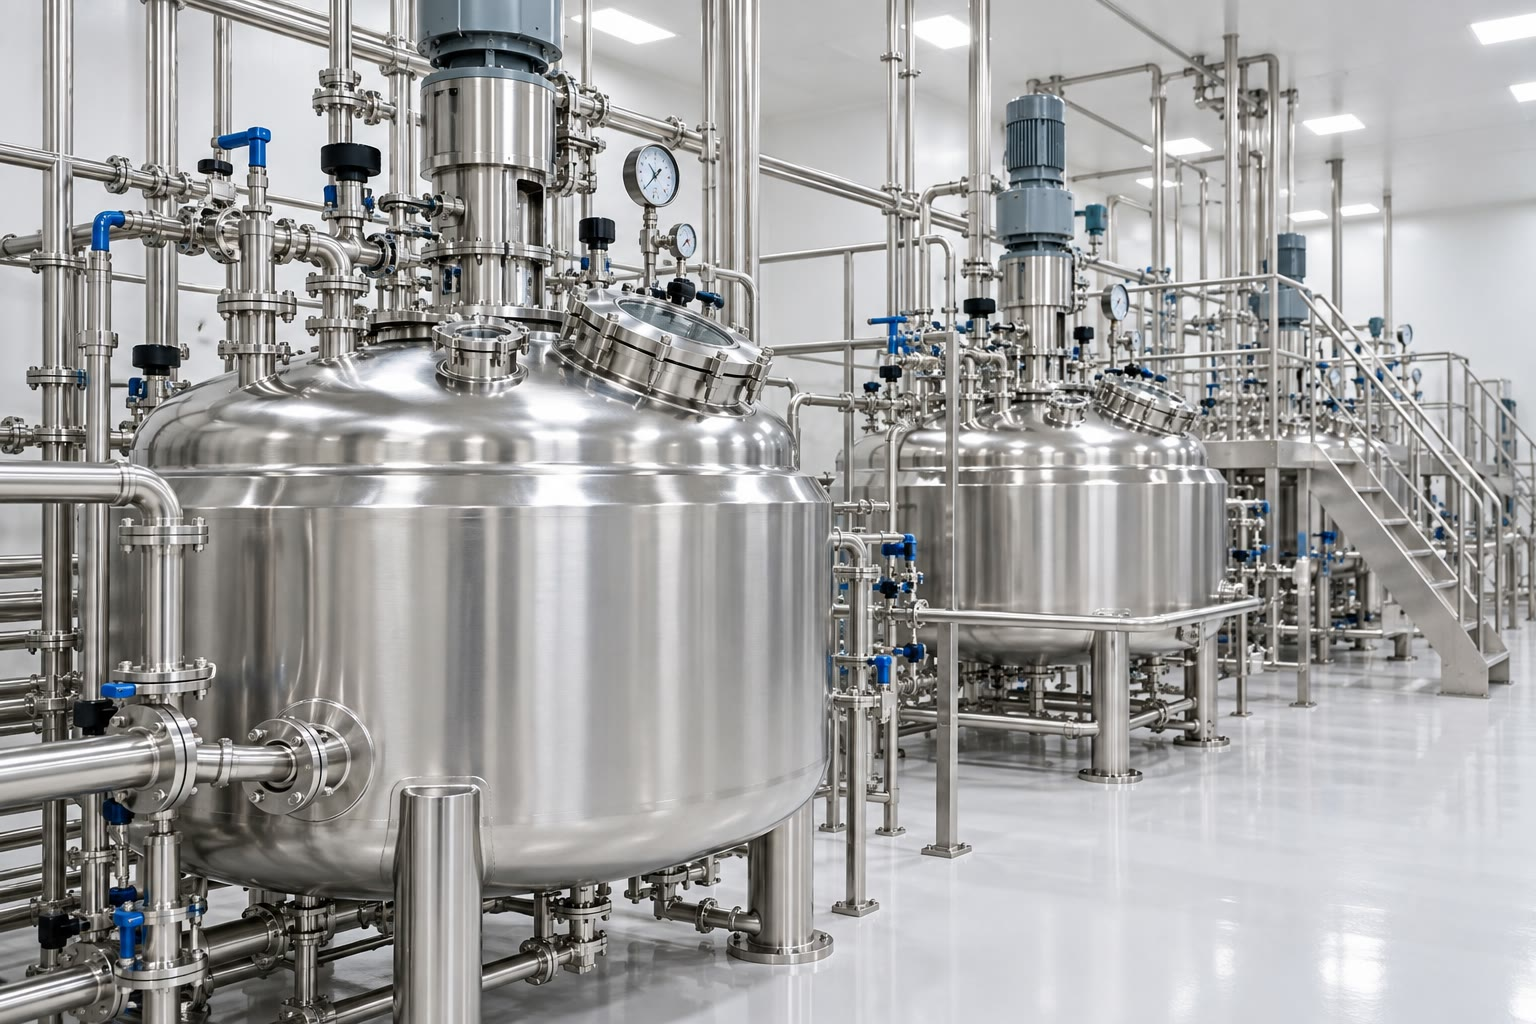
\includegraphics[width=0.55\linewidth]{images/book1/ai/g10-pharma-reactor.jpg}

{\small Steel reactors in a pharmaceutical plant: a laboratory \omterm{def:g10:synthesis-yield:synthesis}{synthesis},
scaled up a millionfold.}
\end{omfigure}

\section{The steps of a synthesis}

\begin{definition}[Synthesis, crude product]\label{def:g10:synthesis-yield:synthesis}
A \emph{synthesis}\index{synthesis} is the preparation of a \omterm{def:g6:pure-substances-and-mixtures:species}{chemical
species} by one or several \omterm{def:g7:chemical-reactions:reaction}{chemical reactions}, starting from other
species. The solid or liquid recovered straight from the reaction
\omterm{def:g6:pure-substances-and-mixtures:mixture}{mixture}, before any purification, is the \emph{crude
product}\index{crude product}: it still contains \omterm{def:g7:chemical-reactions:reactant}{reactants}, by-products
and \omterm{def:g6:solutions-and-solubility:solute}{solvent}.
\end{definition}

\begin{method}[Planning a synthesis]\label{met:g10:synthesis-yield:plan}
A \omterm{def:g10:synthesis-yield:synthesis}{synthesis} is carried out in four steps:
\begin{enumerate}
  \item \textbf{Reaction}: \omterm{def:g2:mixing-and-dissolving:mix}{mix} the \omterm{def:g7:chemical-reactions:reactant}{reactants} in the right amounts, often
        with one in excess, and heat if needed.
  \item \textbf{Isolation}: separate the \omterm{def:g10:synthesis-yield:synthesis}{crude product} from the reaction
        \omterm{def:g6:pure-substances-and-mixtures:mixture}{mixture} (filtration, \omterm{def:g10:chemical-species:extraction}{extraction}).
  \item \textbf{Purification}: remove the impurities from the \omterm{def:g10:synthesis-yield:synthesis}{crude
        product} (\omterm{def:g10:synthesis-yield:recrystallisation}{recrystallisation} for a solid, \omterm{def:g10:chemical-species:distillation}{distillation} for a
        liquid).
  \item \textbf{Analysis}: check the identity and the purity of the
        product (melting point, chromatography), then weigh it and
        compute the \omterm{def:g10:synthesis-yield:yield}{yield}.
\end{enumerate}
\end{method}

\begin{example}[Making aspirin]\label{ex:g10:synthesis-yield:aspirin}
Salicylic acid reacts with ethanoic anhydride (also called acetic
anhydride) to give aspirin and ethanoic acid:
\[
  \ce{C7H6O3 + C4H6O3 -> C9H8O4 + C2H4O2}
\]
\[
  \text{salicylic acid} + \text{ethanoic anhydride} \longrightarrow
  \text{aspirin} + \text{ethanoic acid}.
\]
The anhydride is put in excess, so that all the salicylic acid reacts;
the ethanoic acid formed is a by-product.
\end{example}

\begin{omfigure}
\setchemfig{atom sep=1.7em}
\begin{tabular}{@{}c@{\enspace}c@{\enspace}c@{\enspace}c@{\enspace}c@{\enspace}c@{\enspace}c@{}}
\chemfig{*6(-=-(-COOH)=(-OH)-=)} & $+$ &
\chemfig{H_3C-C(=[2]O)-O-C(=[2]O)-CH_3} & $\longrightarrow$ &
\chemfig{*6(-=-(-COOH)=(-O-[:150]C(=[:90]O)-[:210]H_3C)-=)} & $+$ &
\chemfig{H_3C-C(=[2]O)-OH} \\[2pt]
\small salicylic acid & & \small ethanoic anhydride & &
\small aspirin & & \small ethanoic acid
\end{tabular}\par\medskip

{\small The making of aspirin, in drawn formulas (each corner of the
hexagon is a carbon \omterm{def:g7:atoms-and-molecules:atom}{atom}, bearing a hydrogen \omterm{def:g7:atoms-and-molecules:atom}{atom} where nothing else is
drawn; a later chapter explains this shorthand). The \ce{-OH}
group on the ring of salicylic acid takes half of the anhydride; the
other half leaves as ethanoic acid.}
\end{omfigure}

\section{Heating under reflux}

\begin{definition}[Heating under reflux]\label{def:g10:synthesis-yield:reflux}
\emph{Heating under reflux}\index{heating under reflux} is heating a
reaction \omterm{def:g6:pure-substances-and-mixtures:mixture}{mixture} in a flask topped by a vertical condenser: the vapours
rise, cool in the condenser, and the liquid flows back into the flask.
\end{definition}

\begin{proposition}[Why reflux]\label{prop:g10:synthesis-yield:why-reflux}
Heating makes most reactions faster; reflux allows heating for as long
as needed at the boiling temperature of the \omterm{def:g6:pure-substances-and-mixtures:mixture}{mixture} without losing any
\omterm{def:g7:chemical-reactions:reactant}{reactant}, product or \omterm{def:g6:solutions-and-solubility:solute}{solvent} as vapour.
\end{proposition}

\begin{proof}
The temperature of a boiling liquid cannot rise above its boiling point,
and every vapour that escapes the liquid is condensed and returned:
nothing leaves the apparatus, which stays open at the top so that no
pressure builds up.
\end{proof}

\begin{omfigure}
\begin{tikzpicture}[font=\small, scale=1.05]
  \pic[transform shape] at (0,0) {heatingmantle};
  \pic[transform shape] at (0,0) {rbflask={0.42}{orange!25}};
  \foreach \p in {(-0.3,0.25), (0.2,0.18), (0.45,0.4), (-0.5,0.5)}
    \fill[black!45] \p circle (0.05);
  \pic[transform shape] at (0,3.0) {condenser};
  \draw[omDef, thick, <-] (0.8,3.825) -- (1.9,3.825) node[right] {water in};
  \draw[omDef, thick, ->] (0.8,5.375) -- (1.9,5.375) node[right] {water out};
  \draw[omProp, thick, <-] (-0.18,5.8) -- (-1.4,6.1) node[left] {open top};
  \draw[omProp, thick, <-] (-0.45,1.2) -- (-2.0,1.6)
    node[left, align=right] {reaction mixture\\ and boiling stones};
  \draw[omProp, thick, <-] (-1.35,-0.2) -- (-2.0,-0.6)
    node[left] {heating mantle};
  \draw[omThm, ->, thick] (-0.05,3.4) -- (-0.05,4.3);
  \draw[omDef, ->, thick] (0.05,4.3) -- (0.05,3.4);
  \node[omThm, anchor=east, font=\footnotesize] at (-0.45,4.6) {vapour rises};
  \node[omDef, anchor=west, font=\footnotesize] at (0.85,4.6) {liquid falls back};
\end{tikzpicture}

{\small \omterm{def:g10:synthesis-yield:reflux}{Heating under reflux}. Cold water enters the jacket of the
condenser at the bottom and leaves at the top, so that the jacket is
always full.}
\end{omfigure}

\begin{remark}[Water in at the bottom]\label{rem:g10:synthesis-yield:water}
Fed from the top, the water would run straight down and leave the
upper part of the jacket filled with \omterm{def:g4:air-a-mixture-of-gases:air}{air}; fed from the bottom, it must
fill the whole jacket before it can leave.
\end{remark}

\section{Isolating and purifying}

\begin{definition}[Vacuum filtration]\label{def:g10:synthesis-yield:vacuum-filtration}
\emph{Vacuum filtration}\index{vacuum filtration} is a filtration in
which the liquid is drawn through the filter paper by suction: a flat
funnel with a perforated plate (a Büchner funnel) sits on a side-arm
flask connected to a vacuum pump.
\end{definition}

\begin{omfigure}
\begin{tikzpicture}[font=\small, scale=1.05]
  \pic[transform shape] (ff) at (0,0) {filterflask={0.12}{orange!20}};
  \fill[black!50] (-0.3,2.45) rectangle (0.3,2.8);
  \pic[transform shape] at (0,2.45) {buchner={black!8}};
  \draw[black!60, line width=2pt] (ff-arm) -- (2.6,2.2);
  \draw[omProp, thick, ->] (2.7,2.2) -- (3.4,2.2) node[right,
    align=left, text=black] {to the\\ vacuum pump};
  \draw[omProp, thick, <-] (0.7,3.8) -- (1.9,4.3) node[right, text=black]
    {crystals on filter paper};
  \draw[omProp, thick, <-] (-0.4,0.15) -- (-1.8,0.6) node[left, text=black]
    {filtrate};
  \draw[omProp, thick, <-] (-0.3,2.6) -- (-1.8,2.9) node[left, text=black]
    {rubber seal};
\end{tikzpicture}

{\small \omterm{def:g10:synthesis-yield:vacuum-filtration}{Vacuum filtration} with a Büchner funnel: the pump draws the
liquid through quickly and leaves the solid almost dry.}
\end{omfigure}

\begin{definition}[Recrystallisation]\label{def:g10:synthesis-yield:recrystallisation}
\emph{Recrystallisation}\index{recrystallisation} purifies a solid by
dissolving it in the smallest possible volume of a hot \omterm{def:g6:solutions-and-solubility:solute}{solvent}, then
letting the solution cool: the product, much less soluble in the cold,
crystallises, while the impurities, present in small amounts, stay
dissolved.
\end{definition}

\begin{method}[Recrystallising a solid]\label{met:g10:synthesis-yield:recrystallise}
\begin{enumerate}
  \item Choose a \omterm{def:g6:solutions-and-solubility:solute}{solvent} in which the product is very soluble hot and
        hardly soluble cold.
  \item Add the hot \omterm{def:g6:solutions-and-solubility:solute}{solvent} little by little to the crude solid, just
        until it has all dissolved.
  \item Let the solution cool slowly, then in an ice bath: crystals
        form.
  \item Collect them by \omterm{def:g10:synthesis-yield:vacuum-filtration}{vacuum filtration}, wash them with a little
        ice-cold \omterm{def:g6:solutions-and-solubility:solute}{solvent}, and dry them.
\end{enumerate}
\end{method}


\begin{omfigure}
\begin{tikzpicture}[font=\small]
  % 1. crude solid + a little hot solvent, on a hot plate
  \pic at (0,0.3) {hotplate};
  \pic at (0,0.3) {erlenmeyer={0.18}{orange!12}};
  \foreach \p in {(-0.4,0.42),(-0.15,0.38),(0.1,0.45),(0.35,0.4),(-0.3,0.55),(0.2,0.6)}
    \fill[brown!60] \p circle (0.06);
  \node[align=center, anchor=north] at (0,-0.15) {1. crude solid,\\ hot solvent};
  % 2. clear hot solution
  \pic at (3,0.3) {hotplate};
  \pic at (3,0.3) {erlenmeyer={0.22}{orange!12}};
  \node[align=center, anchor=north] at (3,-0.15) {2. all dissolved,\\ clear and hot};
  % 3. ice bath: crystals
  \fill[cyan!12, draw=black!40] (5.0,0) rectangle (7.0,1.2);
  \foreach \p in {(5.2,0.9),(6.75,1.0),(5.3,0.3),(6.8,0.25)}
    \draw[black!35, fill=white] \p ++(-0.12,-0.1) rectangle ++(0.24,0.2);
  \pic at (6,0.1) {erlenmeyer={0.2}{orange!8}};
  \foreach \x/\y in {-0.45/0.18,-0.25/0.15,0/0.2,0.25/0.15,0.45/0.2,-0.1/0.3,0.15/0.32,
                     -0.35/0.32,0.35/0.33}
    \fill[white, draw=black!55] (6+\x,0.1+\y) -- ++(0.07,0.06) -- ++(0.07,-0.06)
      -- ++(-0.07,-0.06) -- cycle;
  \node[align=center, anchor=north] at (6,-0.15) {3. cool in ice:\\ crystals form};
  % 4. filter
  \pic at (9,0) {filterflask={0.12}{orange!12}};
  \pic at (9,2.45) {buchner={black!12}};
  \fill[black!50] (8.7,2.45) rectangle (9.3,2.8);
  \node[align=center, anchor=north] at (9,-0.15) {4. vacuum filter,\\ wash cold, dry};
\end{tikzpicture}

{\small \omterm{def:g10:synthesis-yield:recrystallisation}{Recrystallisation} in four steps. The impurities stay dissolved in
the cold \omterm{def:g6:solutions-and-solubility:solute}{solvent} and pass into the \omterm{def:g3:separating-mixtures:filter}{filtrate}.}
\end{omfigure}

\begin{remark}[Losses are unavoidable]\label{rem:g10:synthesis-yield:losses}
% ledger: sol:aspirin-25, sol:aspirin-37
Even cold, the \omterm{def:g6:solutions-and-solubility:solute}{solvent} keeps some product dissolved. Aspirin \omterm{def:g2:mixing-and-dissolving:dissolve}{dissolves}
in water at about \qty{3.3}{g/L} at \qty{25}{\celsius}, three times more
at \qty{37}{\celsius}, and much more when hotter: every millilitre of
\omterm{def:g3:separating-mixtures:filter}{filtrate} and of washing water carries a little aspirin away. A
\omterm{def:g10:synthesis-yield:recrystallisation}{recrystallisation} buys purity at the price of mass.
\end{remark}

\section{Analysing the product}

\begin{proposition}[Two checks of purity]\label{prop:g10:synthesis-yield:checks}
A synthesised solid is pure, within the limits of these tests, when:
\begin{itemize}
  \item it melts sharply at the melting point given in the tables;
  \item on a \omterm{def:g10:chemical-species:tlc}{thin-layer chromatography} plate, it gives a single spot,
        at the same height as a sample of the \omterm{def:g6:pure-substances-and-mixtures:pure-substance}{pure substance}.
\end{itemize}
\end{proposition}

\begin{proof}
Admitted: an impurity lowers the melting point and spreads it over a
range (\cref{ch:g10:chemical-species}), and a second species usually
travels a different distance on the plate.
\end{proof}

\begin{omfigure}
\begin{tikzpicture}[font=\small, scale=1.3]
  \pic[transform shape] at (0,0) {tlcplate};
  \draw[black!50, dashed] (-0.7,2.7) -- (0.7,2.7);
  % lanes: C crude, R recrystallised, A aspirin, S salicylic acid
  \foreach \x/\l in {-0.5/C,-0.17/R,0.17/A,0.5/S}
    \node[font=\footnotesize, anchor=north] at (\x,0.38) {\l};
  \fill[omDef!70] (-0.5,1.75) ellipse (0.09 and 0.06);
  \fill[omDef!40] (-0.5,1.25) ellipse (0.09 and 0.06);
  \fill[omDef!70] (-0.17,1.75) ellipse (0.09 and 0.06);
  \fill[omDef!70] (0.17,1.75) ellipse (0.09 and 0.06);
  \fill[omDef!70] (0.5,1.25) ellipse (0.09 and 0.06);
  \node[anchor=west, font=\footnotesize] at (0.85,2.7) {solvent front};
  \node[anchor=west, font=\footnotesize] at (0.85,0.4) {start line};
\end{tikzpicture}

{\small Chromatography of the \omterm{def:g10:synthesis-yield:synthesis}{crude product} (C) and the recrystallised
product (R) beside pure aspirin (A) and salicylic acid (S), seen under
ultraviolet light. The \omterm{def:g10:synthesis-yield:synthesis}{crude product} still holds salicylic acid; the
recrystallised one does not.}
\end{omfigure}

\section{Yield}

\begin{definition}[Yield]\label{def:g10:synthesis-yield:yield}
The \emph{yield}\index{yield} $\eta$ of a \omterm{def:g10:synthesis-yield:synthesis}{synthesis} is the ratio of the
amount of product actually obtained, pure and dry, to the maximum
amount the \omterm{def:g10:reaction-progress-table:limiting}{limiting reactant} could give:
\[
  \eta = \frac{n_{\text{obtained}}}{n_{\max}} ,
\]
usually given as a percentage.
\end{definition}

\begin{proposition}[Yield from masses]\label{prop:g10:synthesis-yield:masses}
Since obtained and maximum amounts concern the same product, of \omterm{def:g10:the-mole:molar-mass}{molar
mass} $M$, the \omterm{def:g10:synthesis-yield:yield}{yield} is also the ratio of masses:
\[
  \eta = \frac{m_{\text{obtained}}}{m_{\max}},
  \qquad m_{\max} = n_{\max} \times M,
\]
where $n_{\max}$ comes from the \omterm{def:g10:reaction-progress-table:extent}{progress table}, at $x = x_{\max}$.
\end{proposition}

\begin{proof}
$m_{\text{obtained}} / m_{\max} = (n_{\text{obtained}} M) / (n_{\max} M)
= n_{\text{obtained}} / n_{\max}$.
\end{proof}

\begin{example}[Yield of a small synthesis]\label{ex:g10:synthesis-yield:small}
% ledger: aw:C, aw:H, aw:O
\qty{1.38}{g} of salicylic acid ($M = \qty{138.0}{g/mol}$), that is
\qty{0.0100}{mol}, react with excess ethanoic anhydride. The maximum
amount of aspirin is \qty{0.0100}{mol}, that is
$0.0100 \times 180.0 = \qty{1.80}{g}$. If \qty{1.35}{g} of pure dry
aspirin are obtained, $\eta = 1.35 / 1.80 = 0.75$, a \omterm{def:g10:synthesis-yield:yield}{yield} of
\qty{75}{\percent}.
\end{example}

\begin{remark}[Why yields are below 100 \%]\label{rem:g10:synthesis-yield:below}
Product is lost at every step: stuck on glassware, dissolved in the
\omterm{def:g3:separating-mixtures:filter}{filtrate} and the washings, left behind in a \omterm{def:g10:synthesis-yield:recrystallisation}{recrystallisation}; some
reactions also give side products, or stop before the \omterm{def:g10:reaction-progress-table:limiting}{limiting reactant}
is used up. A \omterm{def:g10:synthesis-yield:yield}{yield} above \qty{100}{\percent} always signals an error,
most often a product weighed while still wet or impure.
\end{remark}

\begin{inthelab}[Making aspirin]
In a dry flask, the teacher \omterm{def:g2:mixing-and-dissolving:mix}{mixes} salicylic acid with an excess of
ethanoic anhydride and a few drops of an acid that speeds up the
reaction, and heats the \omterm{def:g6:pure-substances-and-mixtures:mixture}{mixture} under reflux in a water bath at about
\qty{80}{\celsius} for a quarter of an hour. After cooling, cold water
is added: the excess anhydride reacts with it, and the aspirin, hardly
soluble in cold water, comes out as white crystals. These are collected
by \omterm{def:g10:synthesis-yield:vacuum-filtration}{vacuum filtration}, recrystallised, dried, weighed, and their melting
point is measured.
\end{inthelab}

\begin{safety}{\ghs[0.82cm]{GHS02}\ghs[0.82cm]{GHS05}\ghs[0.82cm]{GHS06}\ghs[0.82cm]{GHS07}}
% ledger: ghs:acetic-anhydride, ghs:salicylic, ghs:aspirin
Ethanoic anhydride is flammable, harmful if swallowed or inhaled, and causes severe burns
of the skin and the eyes: it is handled by the teacher, under a fume
hood, with gloves and goggles. Salicylic acid is harmful if swallowed and
can damage the eyes. The aspirin made in a laboratory is never taken as
a medicine.
\end{safety}

\begin{omfigure}
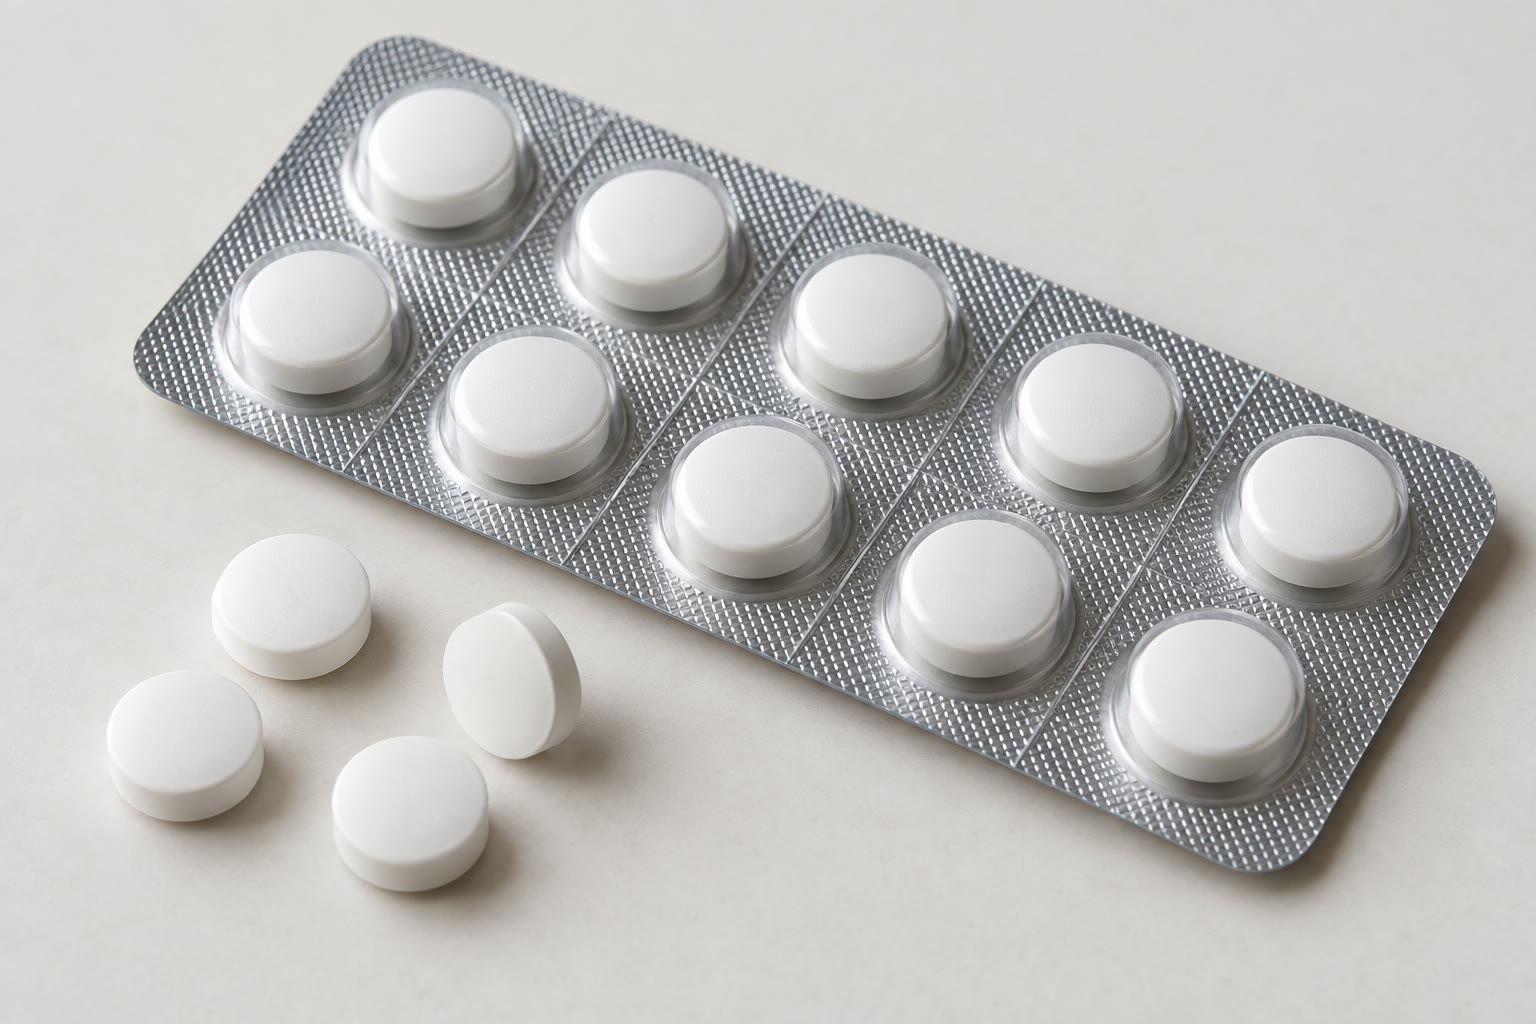
\includegraphics[width=0.45\linewidth]{images/book1/ai/g10-aspirin-tablets.jpg}

{\small Aspirin tablets: each holds a weighed mass of the \omterm{def:g6:pure-substances-and-mixtures:pure-substance}{pure substance},
mixed with a binder.}
\end{omfigure}

\section{Exercises}


\begin{exercise}[$\star$]\label{exo:g10:synthesis-yield:1}
A \omterm{def:g10:synthesis-yield:synthesis}{synthesis} could give at most \qty{5.0}{g} of product; \qty{4.2}{g} of
pure dry product are obtained. Compute the \omterm{def:g10:synthesis-yield:yield}{yield}.
\end{exercise}

\begin{exercise}[$\star$]\label{exo:g10:synthesis-yield:2}
Put these steps of a \omterm{def:g10:synthesis-yield:synthesis}{synthesis} in order: measuring the melting point;
\omterm{def:g10:synthesis-yield:reflux}{heating under reflux}; \omterm{def:g10:synthesis-yield:recrystallisation}{recrystallisation}; \omterm{def:g10:synthesis-yield:vacuum-filtration}{vacuum filtration} of the \omterm{def:g10:synthesis-yield:synthesis}{crude
product}; weighing the \omterm{def:g7:chemical-reactions:reactant}{reactants}.
\end{exercise}

\begin{exercise}[$\star$]\label{exo:g10:synthesis-yield:3}
In a reflux set-up, why is the cooling water fed into the condenser at
the bottom? Why is the top of the condenser left open?
\end{exercise}

\begin{exercise}[$\star$]\label{exo:g10:synthesis-yield:4}
What two properties must a \omterm{def:g6:solutions-and-solubility:solute}{solvent} have to recrystallise a product? Where
do the impurities end up?
\end{exercise}

\begin{exercise}[$\star$]\label{exo:g10:synthesis-yield:5}
% ledger: mp:aspirin
A sample of synthesised aspirin melts between \qty{124}{\celsius} and
\qty{130}{\celsius}. Pure aspirin melts at about \qty{135}{\celsius}. Is
the sample pure? What should be done?
\end{exercise}

\begin{exercise}[$\star\star$]\label{exo:g10:synthesis-yield:6}
\qty{2.00}{g} of salicylic acid react with excess ethanoic anhydride;
\qty{2.03}{g} of pure dry aspirin are obtained. Compute the maximum mass
of aspirin and the \omterm{def:g10:synthesis-yield:yield}{yield}.
\end{exercise}

\begin{exercise}[$\star\star$]\label{exo:g10:synthesis-yield:7}
A student weighs her aspirin while it is still wet and finds a \omterm{def:g10:synthesis-yield:yield}{yield} of
\qty{104}{\percent}. Explain. Would weighing the \omterm{def:g10:synthesis-yield:synthesis}{crude product},
unpurified but dry, give a \omterm{def:g10:synthesis-yield:yield}{yield} that is too high or too low compared
with the true \omterm{def:g10:synthesis-yield:yield}{yield}?
\end{exercise}

\begin{exercise}[$\star\star$]\label{exo:g10:synthesis-yield:8}
Give two advantages of a \omterm{def:g10:synthesis-yield:vacuum-filtration}{vacuum filtration} over an ordinary filtration
through a paper cone, for collecting crystals.
\end{exercise}

\begin{exercise}[$\star\star$]\label{exo:g10:synthesis-yield:9}
On a chromatography plate the \omterm{def:g6:solutions-and-solubility:solute}{solvent} front has moved \qty{5.0}{cm}. The
spot of a synthesised product has moved \qty{3.1}{cm}, that of pure
aspirin \qty{3.1}{cm}, that of salicylic acid \qty{2.2}{cm}. Compute the
three \omterm{def:g10:chemical-species:retention-factor}{retention factors}. What can be concluded about the product?
\end{exercise}

\begin{exercise}[$\star\star$]\label{exo:g10:synthesis-yield:10}
The \omterm{def:g6:solutions-and-solubility:solubility}{solubility} of a product in two \omterm{def:g6:solutions-and-solubility:solute}{solvents} is:
\begin{center}
\begin{tabular}{lcc}
\hline
\omterm{def:g6:solutions-and-solubility:solute}{solvent} & cold (\qty{20}{\celsius}) & hot (near boiling) \\
\hline
A & \qty{2}{g/L} & \qty{150}{g/L} \\
B & \qty{80}{g/L} & \qty{120}{g/L} \\
\hline
\end{tabular}
\end{center}
Which \omterm{def:g6:solutions-and-solubility:solute}{solvent} is better for a \omterm{def:g10:synthesis-yield:recrystallisation}{recrystallisation}? For \qty{3.0}{g} of
\omterm{def:g10:synthesis-yield:synthesis}{crude product}, about what volume of hot \omterm{def:g6:solutions-and-solubility:solute}{solvent} is needed, and what mass
at most stays dissolved once cold?
\end{exercise}

\begin{exercise}[$\star\star$]\label{exo:g10:synthesis-yield:11}
Why is the round-bottom flask of a reflux set-up never more than half
full? Why are boiling stones added?
\end{exercise}

\begin{exercise}[$\star\star\star$]\label{exo:g10:synthesis-yield:12}
A medicine is made in two steps, of \omterm{def:g10:synthesis-yield:yield}{yields} \qty{80}{\percent} and
\qty{70}{\percent}. What is the overall \omterm{def:g10:synthesis-yield:yield}{yield}? What would it be for
three steps of \qty{90}{\percent} each? Why do chemists try to make
medicines in as few steps as possible?
\end{exercise}

\begin{exercise}[$\star\star\star$]\label{exo:g10:synthesis-yield:13}
% ledger: sol:aspirin-25
Aspirin \omterm{def:g2:mixing-and-dissolving:dissolve}{dissolves} in water at about \qty{3.3}{g/L} at
\qty{25}{\celsius}. Crystals are washed with \qty{50}{mL} of water at
that temperature. What mass of aspirin may be lost at most? Why is the
washing water cooled in ice first?
\end{exercise}

\begin{exercise}[$\star\star\star$]\label{exo:g10:synthesis-yield:14}
\qty{2.76}{g} of salicylic acid are mixed with \qty{0.0500}{mol} of
ethanoic anhydride. After the reaction, water is added and destroys the
excess anhydride: \ce{C4H6O3 + H2O -> 2C2H4O2}.
\begin{enumerate}
  \item Fill the \omterm{def:g10:reaction-progress-table:extent}{progress table} of the \omterm{def:g10:synthesis-yield:synthesis}{synthesis}; what amount of
        anhydride is left?
  \item What total amount of ethanoic acid is present at the end?
\end{enumerate}
\end{exercise}

\begin{exercise}[$\star\star\star$]\label{exo:g10:synthesis-yield:15}
A factory must make \qty{1.00}{t} of aspirin, with an overall \omterm{def:g10:synthesis-yield:yield}{yield} of
\qty{85}{\percent} from salicylic acid. What mass of salicylic acid must
it buy?
\end{exercise}

\section{Problem: Making Aspirin}

\begin{problem}[{Weekend problem --- from three grams of salicylic acid
to a jar of pure aspirin: what is the yield?}]
\label{pb:g10:synthesis-yield:1}
% ledger: rho:acetic-anhydride, mp:aspirin, mp:salicylic, sol:aspirin-25, aw:C, aw:H, aw:O
A class makes aspirin. In the flask: \qty{3.0}{g} of salicylic acid and
\qty{6.0}{mL} of ethanoic anhydride, of density \qty{1.08}{g/mL}, with a
few drops of acid; the \omterm{def:g6:pure-substances-and-mixtures:mixture}{mixture} is heated under reflux. The \omterm{def:g10:synthesis-yield:synthesis}{crude product}
collected by \omterm{def:g10:synthesis-yield:vacuum-filtration}{vacuum filtration} weighs \qty{3.6}{g} wet and \qty{3.3}{g}
once dry. After \omterm{def:g10:synthesis-yield:recrystallisation}{recrystallisation} and drying, \qty{2.7}{g} of white
crystals remain.

\medskip
\noindent\textbf{Part I --- The reaction.}
\begin{enumerate}
  \item Check that the equation
        \ce{C7H6O3 + C4H6O3 -> C9H8O4 + C2H4O2} is balanced.
  \item Compute the molar masses of salicylic acid, ethanoic anhydride,
        aspirin and ethanoic acid.
  \item Name the \omterm{def:g7:chemical-reactions:reactant}{reactants}, the product wanted and the by-product.
  \item Why is the \omterm{def:g6:pure-substances-and-mixtures:mixture}{mixture} heated under reflux rather than in an open
        flask?
\end{enumerate}

\medskip
\noindent\textbf{Part II --- The maximum mass.}
\begin{enumerate}[resume]
  \item Compute the initial amount of salicylic acid.
  \item Compute the mass, then the amount, of ethanoic anhydride.
  \item Fill the \omterm{def:g10:reaction-progress-table:extent}{progress table}. Which \omterm{def:g7:chemical-reactions:reactant}{reactant} is limiting? Give
        $x_{\max}$.
  \item Deduce the maximum mass of aspirin.
  \item Why is the anhydride, rather than the salicylic acid, put in
        excess?
\end{enumerate}

\medskip
\noindent\textbf{Part III --- Isolating and purifying.}
\begin{enumerate}[resume]
  \item Why can the wet mass, \qty{3.6}{g}, not be used to compute a
        \omterm{def:g10:synthesis-yield:yield}{yield}?
  \item Compute the \omterm{def:g10:synthesis-yield:yield}{yield} of crude dry product.
  \item Why does the \omterm{def:g10:synthesis-yield:recrystallisation}{recrystallisation} lower the mass?
  \item The crystals were washed with \qty{30}{mL} of water at
        \qty{25}{\celsius}, where aspirin \omterm{def:g2:mixing-and-dissolving:dissolve}{dissolves} at about
        \qty{3.3}{g/L}. What mass could at most be lost this way?
  \item Compute the \omterm{def:g10:synthesis-yield:yield}{yield} of pure product.
\end{enumerate}

\medskip
\noindent\textbf{Part IV --- Checking the product.}
\begin{enumerate}[resume]
  \item The recrystallised crystals melt sharply at \qty{135}{\celsius}.
        What does this show?
  \item The \omterm{def:g10:synthesis-yield:synthesis}{crude product} melted between \qty{120}{\celsius} and
        \qty{131}{\celsius}. What does this show?
  \item On a chromatography plate, the \omterm{def:g10:synthesis-yield:synthesis}{crude product} gives two spots,
        one at the height of pure aspirin and one at the height of
        salicylic acid; the recrystallised product gives one spot, at
        the height of aspirin. Conclude.
  \item The spot of the recrystallised product moved \qty{3.1}{cm} and
        the \omterm{def:g6:solutions-and-solubility:solute}{solvent} front \qty{5.0}{cm}. Compute its \omterm{def:g10:chemical-species:retention-factor}{retention factor}.
  \item Between the reaction and the \omterm{def:g10:synthesis-yield:recrystallisation}{recrystallisation}, which part of the
        work lost more aspirin?
  \item State the final answer: what is the \omterm{def:g10:synthesis-yield:yield}{yield} of the \omterm{def:g10:synthesis-yield:synthesis}{synthesis}?
\end{enumerate}
\end{problem}
